\documentclass[a4paper, 11pt]{article}
    \usepackage{comment} % enables the use of multi-line comments (\ifx \fi) 
    \usepackage{lipsum} %This package just generates Lorem Ipsum filler text. 
    \usepackage{fullpage} % changes the margin
    % Used for importing figures
    \usepackage{graphicx}
    \usepackage{wrapfig}
    \usepackage{float}
    
\begin{document}

%Header-Make sure you update this information!!!!
\noindent
\large\textbf{Lab 1} \hfill \textbf{Zach Colbert} \\
\normalsize PH 411 \hfill Lab Partner: Michael Trumbull \\
Electronics  \hfill Lab Date: 21-26 Sept 2017 \\
McIntyre \hfill Due Date: 5 Oct 2017

\section{Part 1}
    \subsection{Introduction}


        %     Provide introductory discussion of what you are studying. What are you going to
        %     measure? What can you learn from making these measurements? To obtain nice flow in
        %     the introduction it is often better to discuss broad concepts first and then narrow the focus
        %     to specific phenomena. A few sentences are usually sufficient.


        For the first part of the lab, we took a couple of different approaches to measuring the resistance of a \(1.6\ k\Omega \) resistor. We also sought to determine if the resistor behaves ohmically---that is, if it obeys Ohm's Law. We accomplished this by comparing the voltage drop across the resistor and current through the resistor in a simple circuit.

    \subsection{Experimental}

        %     a) Discuss theoretical models and provide any relevant equations.
        %     b) Draw a circuit diagram showing your experimental setup. You may hand draw your
        %     circuit diagrams, or find some program to use. If you find a useful circuit-drawing
        %     program, please let the rest of the class know about it. Label components in the circuit
        %     diagram with symbols/variables, and include numeric values where needed.
        %     c) Discuss specific measuring techniques and experimental designs of the experiment.

        \begin{wrapfigure}{R}{0.4\textwidth}
            \vspace{-25pt}
            \centering
            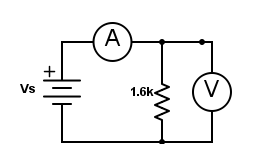
\includegraphics[height=3cm]{PH425-Lab1-1b.png}
            \caption{Resistor in a simple circuit with ammeter and voltmeter.}
            \label{fig:circuit-1b}
        \end{wrapfigure}

        Initially, using a digital multimeter to measure the resistance of our resistor alone (outside of the circuit) was useful for determining what the resistance is. It does not, however show whether the resistor is Ohmic or not---that is, if the element has a constant resistance as current and voltage change. \
        
        By comparing the voltage drop \( V \) across the resistor and the current \(I \) through the resistor, we can look for Ohm's law as a linear function \( V = IR \). The circuit diagram in Figure \ref{fig:circuit-1b} shows how two meters were used to measure these quantities in our simple circuit.

    \subsection{Results}

        % Present results in graphical form. Label graphs with informative titles, and indicate data regions where interesting behavior occurs. Label the axes of graphs clearly and include units.

        \begin{figure}[H]
            \centering
            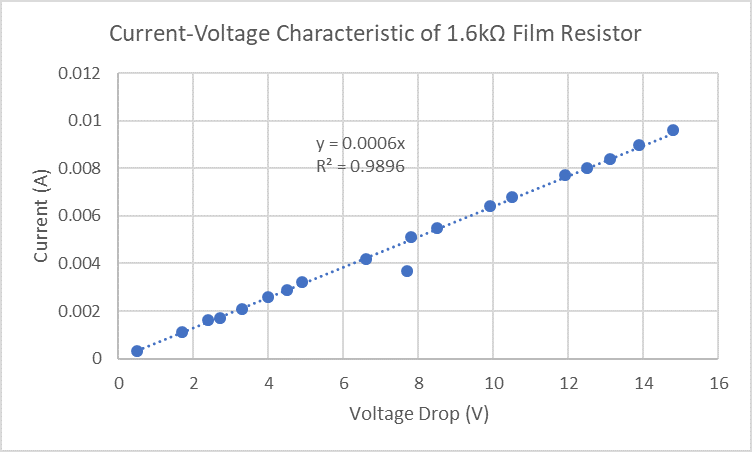
\includegraphics{PH425-Lab1-1b-1.png}
            \caption{Current-Voltage characteristic of the resistor in \ref{fig:circuit-1b}, with trendline for an Ohmic resistor.}
            \label{fig:results-1b}
        \end{figure}
        \newpage

        % Compare results with theoretical expectations. When appropriate, include a theory curve on the data plot, using points for experimental data and lines/curves for theory.

        Figure \ref{fig:results-1b} is a visual comparison of the resistor's behavior to Ohm's law---which is represented as a linear function of voltage across and current through the resistor, \( I = V/R \). \
        
        By that relationship, the slope of the line in Figure \ref{fig:results-1b} is equal to the inverse of the resistance \( R \), which comes out to about \( 1.67 k\Omega \).
        
        % Discuss any error analysis performed.

    \subsection{Conclusion}

        % What did you learn?

        % Was there anything unexpected?

        % What is the general behavior of the circuit in the experiment?

        Most of the data fits nicely along the Ohmic line, except for the single point near 8 volts which falls well outside the expected margin of error \( \pm 0.5 mA \). Despite that extraneous point, the data overall seems to follow the trend we expect for an Ohmic element. \

        % How do your results compare to theory?

        % Summarize the key concepts.

        By obeying Ohm's Law across a range of different voltages and currents, we expect this resistor and similar elements to have reliably constant resistance in other applications.

\section{Part 2}
    \subsection{Introduction}

        % Provide introductory discussion of what you are studying.

        As in Part 1, we used current-voltage characteristics in Part 2 to observe the behavior of three new elements in regards to Ohm's Law: \

        % What are you going to measure?

        \begin{itemize}
            \item Small incandescent light bulb
            \item 1N914 diode
            \item Green light-emitting diode
        \end{itemize}

        % What can you learn from making these measurements?

        The conclusions drawn from Part 2 will be useful in forming intuition about the behavior of these elements, so that we can build more complex circuits with these elements in the future.

    \subsection{Experimental}

        \begin{wrapfigure}{R}{0.4\textwidth}
            \vspace{-25pt}
            \centering
            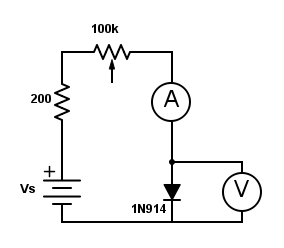
\includegraphics[height=3cm]{PH425-Lab1-2b.png}
            \caption{Resistor in a simple circuit with ammeter and voltmeter.}
            \label{fig:circuit-2}
        \end{wrapfigure}

        % Discuss theoretical models and provide any relevant equations.

        The theoretical model behind Part 2 is the same as in Part 1---a current-voltage characteristic curve for each element allows us to visualize the resistance of the element and compare it to an ideal element that obey's Ohm's Law. \

        % Draw a circuit diagram showing your experimental setup. Label components in the circuit diagram with symbols/variables, and include numeric values where needed.

        The circuit in Figure \ref{fig:circuit-2} shows one of the chosen elements, a 1N914 diode, in series with some current-limiting resistors. Other elements that were tested in Part 2 followed the same model. \

        % Discuss specific measuring techniques and experimental designs of the experiment.

        One change from the procedure of Part 1 is in the source voltage that is applied to the circuit. Because diodes are designed to only allow current to flow in one direction, we took data for positive and negative source voltages (or current, running either direction through the circuit).

    \subsection{Results}

        % Present results in graphical form. Label graphs with informative titles, and indicate data regions where interesting behavior occurs. Label the axes of graphs clearly and include units.

        \begin{figure}[H]
            \centering
            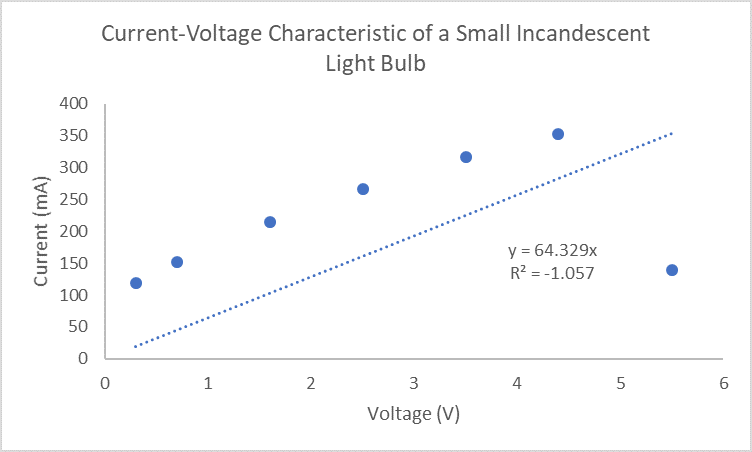
\includegraphics{PH425-Lab1-2a-R.png}
            \caption{Current-Voltage characteristic of the small incandescent bulb, with trendline for an Ohmic resistor.}
            \label{fig:results-2a}
        \end{figure}

        The incandescent bulb showed a fairly linear characteristic curve over most of the applied voltages, but dropped off very rapidly around \( 5 V \). We were not able to resolve data in that part of the curve very well because we did not choose elements---namely our current-limiting potentiometer and power supply---that were precise enough to collect more data points in that region. \
        
        It's also important to note that the current at each data point was not entirely stable. We saw the current at each recorded voltage slowly rise over time.

        \begin{figure}[H]
            \centering
            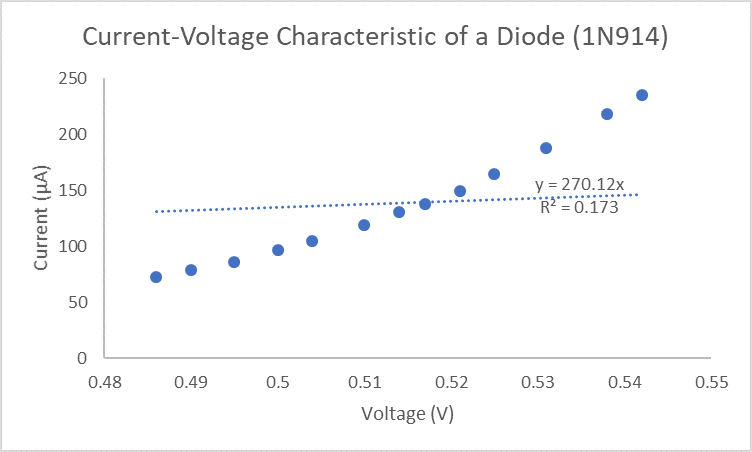
\includegraphics{PH425-Lab1-2b-R.png}
            \caption{Current-Voltage characteristic of the 1N914 diode in \ref{fig:circuit-2}, with trendline for an Ohmic resistor.}
            \label{fig:results-2b}
        \end{figure}

        \begin{figure}[H]
            \centering
            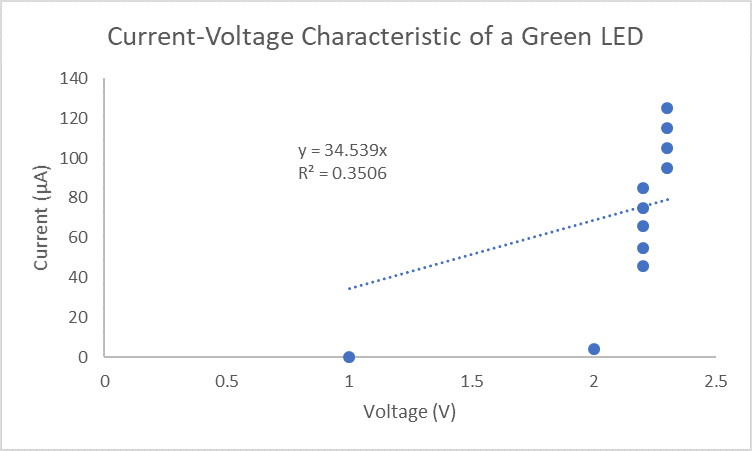
\includegraphics{PH425-Lab1-2c-R.png}
            \caption{Current-Voltage characteristic of the light-emitting diode, with trendline for an Ohmic resistor.}
            \label{fig:results-2c}
        \end{figure}

        % Compare results with theoretical expectations. When appropriate, include a theory curve on the data plot, using points for experimental data and lines/curves for theory.
        
        % Discuss any error analysis performed.

    \subsection{Conclusion}

        % What did you learn?

        % Was there anything unexpected?

        % What is the general behavior of the circuit in the experiment?

        % How do your results compare to theory?

        % Summarize the key concepts.

\section{Part 3}
    \subsection{Introduction}

        % Provide introductory discussion of what you are studying.

        % What are you going to measure?

        % What can you learn from making these measurements?

    \subsection{Experimental}

        % Discuss theoretical models and provide any relevant equations.

        % Draw a circuit diagram showing your experimental setup. Label components in the circuit diagram with symbols/variables, and include numeric values where needed.

        % Discuss specific measuring techniques and experimental designs of the experiment.

    \subsection{Results}

        % Present results in graphical form. Label graphs with informative titles, and indicate data regions where interesting behavior occurs. Label the axes of graphs clearly and include units.

        % Compare results with theoretical expectations. When appropriate, include a theory curve on the data plot, using points for experimental data and lines/curves for theory.
        
        % Discuss any error analysis performed.

    \subsection{Conclusion}

        % What did you learn?

        % Was there anything unexpected?

        % What is the general behavior of the circuit in the experiment?

        % How do your results compare to theory?

        % Summarize the key concepts.

\end{document}
